%% !TEX root = ../Thesis.tex
%% !TEX output_directory
\documentclass[11pt,a4paper,english,greek,twoside]{../Thesis}
\begin{document}
\chapter{Το Υποσύστημα Εξαγωγής Χαρακτηριστικών Όρασης Χαμηλού Επιπέδου}\label{chap:Methodology}
Στο προηγούμενο κεφάλαιο είδαμε τη δομή του συνολικού συστήματος. Ακόμα νωρίτερα, στο ίδιο κεφάλαιο, γνωρίσαμε διάφορες προσεγγίσεις αναγνώρισης δράσεων που χρησιμοποιούν σημασιολογία ή οπτικά χαρακτηριστικά υψηλού επιπέδου. Η αναγνώριση δράσεων με χαρακτηριστικά χαμηλού επιπέδου είναι εξίσου σημαντική και πιθανόν ισχυρή. Διαισθητικά, η πληροφορία κίνησης εξασφαλίζει την ύπαρξη δράσης, την ώρα που απλές επισημειώσεις περιβάλλοντος αδυνατούν να εγγυηθούν κάτι παρόμοιο. Ακόμα περισσότερο, η αναπαράσταση των δράσεων στις ιεραρχικές μεθόδους συχνά προϋποθέτει ισχυρά μοντέλα ταξινομητών χαμηλού επιπέδου. Το παρόν κεφάλαιο οργανώνεται ως εξής: αρχικά γίνεται μια ιστορική ανασκόπηση της αναγνώρισης δράσεων με οπτικά χαρακτηριστικά χαμηλού επιπέδου. Στη συνέχεια παρουσιάζεται η θεωρία της μεθόδου των Πυκνών Τροχιών και των χαρακτηριστικών που χρησιμοποιεί. Αναλύονται επίσης τα χαρακτηριστικά πόζας και η κωδικοποίηση των χαρακτηριστικών για δημιουργία ιστογραμμάτων. Τέλος, παρουσιάζουμε τη δική μας μέθοδο η οποία συνδυάζει όλα τα παραπάνω.


%%%%%%%%%%%%%%%%%%%%%%%%%%%%%%%%%%%%%%%%%%%%%% History
\section{Ιστορικά Στοιχεία}
Η πρώτη απόπειρα μοντελοποίησης των δράσεων σε βίντεο μπορεί να θεωρηθεί η σειρά πειραμάτων του Johansson \cite{johansson_1973} το 1973. Στην εργασία αυτή, συγκεντρώνεται ένα σύνολο δεδομένων με ανθρώπους σε μαύρη ενδυμασία στους κύριους συνδέσμους των οποίων έχουν τοποθετηθεί μικρά φώτα. Σκοπός του πειράματος ήταν η εξέταση του αν η πληροφορία αυτή είναι αρκετή ώστε ένας άνθρωπος να αποφανθεί για την δράση του υποκειμένου. Το 1982 το \cite{webb_1982} είναι η πρώτη εργασία που μελετά την εύρεση της δομής των αντικειμένων από την κίνηση και θεωρείται ότι γέννησε την αναγνώριση δράσεων μέσω συνδέσμων. Η έρευνα εντείνεται από τη δεκαετία του '90 μέχρι και σήμερα, επιτυγχάνοντας αρκετά αξιόλογα αποτελέσματα και εξελίσσοντας πολλαπλές μεθόδους.

\par Η πρώτη προσέγγιση ήταν η λεγόμενη σειριακή (sequential). Η ιδέα είναι ότι μία δράση μπορεί να εκφραστεί ως ακολουθία καταστάσεων των μερών του σώματος. Κάθε frame επομένως περιγράφει μία συγκεκριμένη διάταξη αυτών των μερών. Η αναγνώριση μπορεί να γίνει με Κρυφά Μαρκοβιανά Μοντέλα (Hidden Markov Models, HMM)  όπου μια κατάσταση αντιστοιχεί σε μία συγκεκριμένη πόζα σώματος \cite{yamato_1992}, \cite{starner_1995}. Μια εναλλακτική είναι η χρήση δυναμικού προγραμματισμού για το ταίριασμα δύο ακολουθιών \cite{gavrila_1995}. Η προσέγγιση αυτή εξελίχθηκε με αρκετές παραλλαγές τα επόμενα χρόνια, όπως χρήση συζευγμένων Κρυφών Μαρκοβιανών \cite{oliver_2000} και Ημι-Μαρκοβιανών Μοντέλων \cite{natarajan_2007}, καθώς και Δυναμικών Μπεϋζιανών Δικτύων (Dynamic Bayesian Networks) \cite{park_2004}. Ωστόσο, βασικό μειονέκτημα αυτών των προσεγγίσεων είναι η εξάρτηση από ισχυρά χαρακτηριστικά (features) για τις δράσεις και η αδυναμία διαχωρισμού σύνθετων δράσεων χωρίς πολύ μεγάλο μέγεθος συνόλου δεδομένων εκπαίδευσης.

\par Μια επόμενη προσέγγιση ήταν η χωροχρονική (space-time), η οποία αντιμετωπίζει τα βίντεο σαν τρισδιάστατους όγκους, με την τρίτη διάσταση να αποτελεί τον χρόνο. Εδώ το πρόβλημα είναι το ταίριασμα όγκων ως λύση της ταξινόμησης. Μία λύση σε αυτό ήταν το απευθείας ταίριασμα προτύπων (template matching) όπως στο \cite{bobick_2001} όπου εισάγεται η έννοια των Εικόνων Ιστορίας Κίνησης (Motion History Images) ως μια σταθμισμένη προβολή ενός χωροχρονικού όγκου προσκηνίου. Στο \cite{ke_2007} το ταίριασμα γίνεται σε υποόγκους του βίντεο και τα επιμέρους σκορ συνδυάζονται. Η ιδέα εξελίχθηκε στην εξαγωγή χωροχρονικών χαρακτηριστικών από τα βίντεο, καθολικά (global), όπως οπτική ροή \cite{efros_2003}, αλλά και τοπικά, όπως στο \cite{laptev_2004} και αραιά, όπως τα κυβοειδή του \cite{dollar_2005}. Οι προσεγγίσεις αυτές εξελίχθηκαν σημαντικά στα επόμενα χρόνια \cite{laptev_2008}, ώστε να λαμβάνουν υπόψιν τους τις χρονικές εξαρτήσεις των χαρακτηριστικών \cite{savarese_2008}, \cite{wong_2007}.

\begin{figure}
  \centering
  \noindent\makebox[\textwidth]{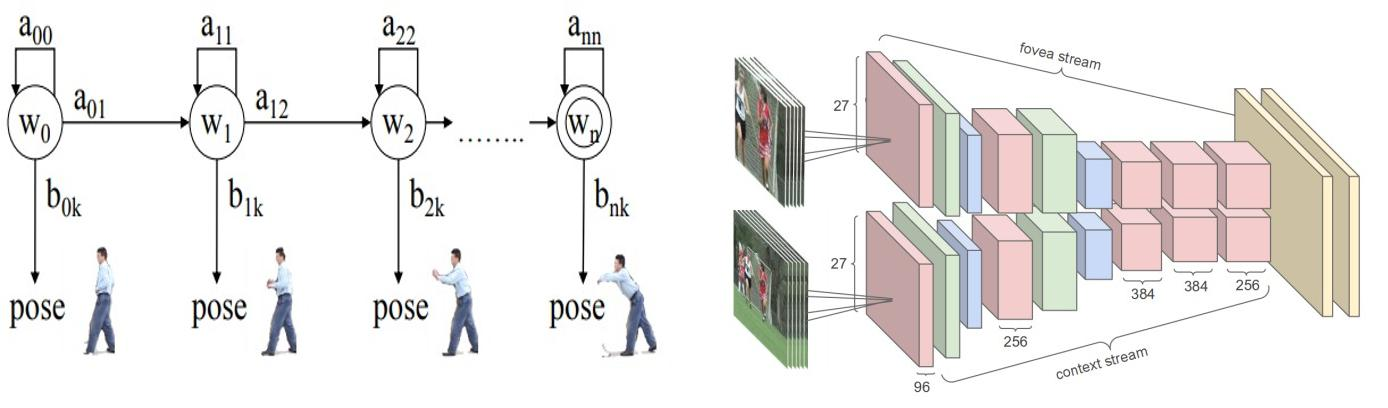
\includegraphics[scale=0.3]{{Images/chap3Karpathy}.jpg}}
  \caption{Η εξέλιξη της Αναγνώρισης δράσεων με τεχνικές που στηρίζονται αποκλειστικά στην οπτική αντίληψη, από τις ισχυρές υποθέσεις στην αφηρημένη δομή δικτύου. $\textbf{Αριστερά}$: ένα παράδειγμα σειριακής προσέγγισης που κάνει χρήση Κρυφού Μαρκοβιανού Μοντέλου για να αναπαραστήσει την απλή δράση "Σπρώχνω" με καταστάσεις που αντιστοιχούν σε ενδιάμεσες στάσεις σώματος. Εικόνα από \cite{cvpr_2014}. $\textbf{Δεξιά}$: Δομή Συνελικτικού Νευρωνικού Δικτύου για ανάλυση αθλητικών αγώνων από την εργασία \cite{karpathy_2014}.}
  \label{fig:chap3Karpathy}
\end{figure}

\par Η εξέλιξη των μεθόδων χωροχρονικών χαρακτηριστικών ήταν συνυφασμένη με την απομάκρυνση από τις αναλύσεις σχήματος και πόζας. Η κίνηση θεωρήθηκε το κύριο στοιχείο που καθορίζει τη δράση. Από τους τύπους χαρακτηριστικών, αυτά που επικράτησαν ήταν τα τοπικά, καθώς περιγράφουν με ευρωστία τα κύρια συστατικά της κίνησης. Ένα πολύ σημαντικό βήμα προς αυτή την κατεύθυνση ήταν η εργασία των \cite{wang_2011} που εισήγαγε τις Πυκνές Τροχιές. Η μέθοδος αυτή βελτιώθηκε και εξελίχθηκε \cite{wang_2013} επιτυγχάνοντας ποσοστά ακριβείας βελτιωμένα κατά μεγάλο περιθώριο σε πολλές βάσεις βίντεο. Άξια αναφοράς η εργασία των \cite{kantorov_2014} η οποία εστιάζει στην αποδοτικότητα των αλγορίθμων αναγνώρισης δράσεων και παρέχει αλγορίθμους τάξεις μεγέθους γρηγορότερους από τις Πυκνές Τροχιές με κάποιο κόστος στην ακρίβεια. Άλλες μέθοδοι αξιοποιούν και δεδομένα βάθους \cite{chen_2013}, ενώ, τελευταία, τα Συνελικτικά Νευρωνικά Δίκτυα (Convolutional Neural Networks, CNN) μπήκαν επίσης στο πεδίο της αναγνώρισης δράσεων με το \cite{karpathy_2014} και πρωταγωνιστούν στην εξέλιξη και τα state-of-the-art αποτελέσματα \cite{cherian_2017}.


%%%%%%%%%%%%%%%%%%%%%%%%%%%%%%%%%%%%%%%%%%%%%%% Theory
\section{Θεωρητικό Υπόβαθρο}

%%%%%%%%%%%%%%%%%%%%%%%% Dense Trajectories
\subsection{Η Μέθοδος των Πυκνών Τροχιών}
Η μέθοδος των Πυκνών Τροχιών αποτελεί μια state-of-the-art μέθοδο για αναγνώριση δράσης σε βίντεο αξιοποιώντας μόνο οπτική πληροφορία. Ως Πυκνές Τροχιές ορίζουμε τη χωροχρονική τροχιά των σημείων ενδιαφέροντος πάνω σε ένα πυκνά δειγματοληπτημένο πλέγμα. Η ιδέα βασίζεται στην επιτυχία της πυκνής δειγματοληψίας \cite{wang_2009} στην εξαγωγή σημείων ενδιαφέροντος και των μεθόδων ανίχνευσης κίνησης και προσκηνίου και προτάθηκε στο \cite{wang_2011}. Η μέθοδος απέκτησε δημοφιλία λόγω της απλότητας, της ταχύτητας αλλά και της αποτελεσματικότητάς της, καθώς βελτίωνε τα αποτελέσματα αναγνώρισης σε όλα τα σύνολα δεδομένων. Επιπλέον, έχει τη δυνατότητα να αναιρεί την υπόθεση της σταθερής κάμερας, μοντελοποιώντας την κίνησή της. Μάλιστα, στο \cite{wang_2013} επεκτείνεται το μοντέλο και πετυχαίνει καλύτερη αντιστάθμιση της κίνησης της κάμερας με αντίστοιχη βελτίωση στην ακρίβεια του συστήματος. Στη συνέχεια θα παρουσιάσουμε συνοπτικά τα κυριότερα σημεία της μεθόδου.

\par Οι πυκνές τροχιές εξάγονται σε πολλαπλές χωρικές κλίμακες, μέχρι 8 το πλήθος, οι οποίες προκύπτουν από υποδειγματοληψία της προηγούμενής τους κλίμακας (με αρχική κλίμακα 1, δηλαδή αρχική εικόνα την αυθεντική) κατά έναν παράγοντα $1/\sqrt{2}$. Τα σημεία ενδιαφέροντος εξάγονται από ένα χωρικό πλέγμα με κατάλληλο βήμα W pixels, έτσι ώστε να μπορεί να καλυφθεί όλη η εικόνα. Παρακολουθούμε τα σημεία ενδιαφέροντος αυτά σε κάθε κλίμακα ανεξάρτητα, με την κίνηση κάθε σημείου $P_t=(x_t,y_t)$ από το frame $t$ στο frame $t+1$ να προσεγγίζεται από την εξίσωση:

\begin{equation}\label{eq:pointDense}
    P_{t+1}=P_t+(M*\omega) |_{(\bar{x}_t,\bar{y}_t)}
\end{equation}

όπου $Μ$ ένα φίλτρο διαμέσου (median) διάστασης $3 \times 3$, $(\bar{x}_t,\bar{y}_t)$ η θέση του σημείου στο frame $t$ κατόπιν στρογγυλοποίησης των συντεταγμένων και $\omega$ το πεδίο πυκνής οπτικής ροής, υπολογισμένο με τη μέθοδο του Farneback \cite{farneback_2003}. Τα σημεία $(P_t, P_{t+1}, \dots )$ συνενώνονται για να σχηματίσουν μια ακολουθία που ονομάζεται τροχιά. Καθώς οι τροχιές έχουν την τάση να ολισθαίνουν κατά τη διάρκεια ενός βίντεο, το μήκος τους περιορίζεται σε $L = 15$ σημεία και ένα σημείο παύει να παρακολουθείται όταν η τροχιά του ξεπεράσει το προκαθορισμένο αυτό μήκος. Ταυτόχρονα, για να εξασφαλιστεί η πυκνή κάλυψη του βίντεο, σε κάθε frame γίνεται έλεγχος αν παρακολουθείται κάποιο σημείο εντός μιας γειτονιάς $W \times W$ σημείων από τις αρχικές. Αν δεν βρεθεί τέτοιο σημείο, δειγματοληπτείται ένα νέο και προστίθεται στη διαδικασία παρακολούθησης. Τροχιές που είναι στατικές αφαιρούνται, μιας και δεν περιέχουν καμία πληροφορία που σχετίζεται με κίνηση εντός του βίντεο, ενώ τροχιές που παρουσιάζουν απότομες μετατοπίσεις μεταξύ δύο διαδοχικών frame επίσης εκτοπίζονται. Θα σταθούμε σε αυτό το σημείο για να παρουσιάσουμε κάποια βήματα υπολογισμού των τροχιών και σχεδιαστικές επιλογές με μεγαλύτερη λεπτομέρεια.

\begin{figure}
  \centering
  \noindent\makebox[\textwidth]{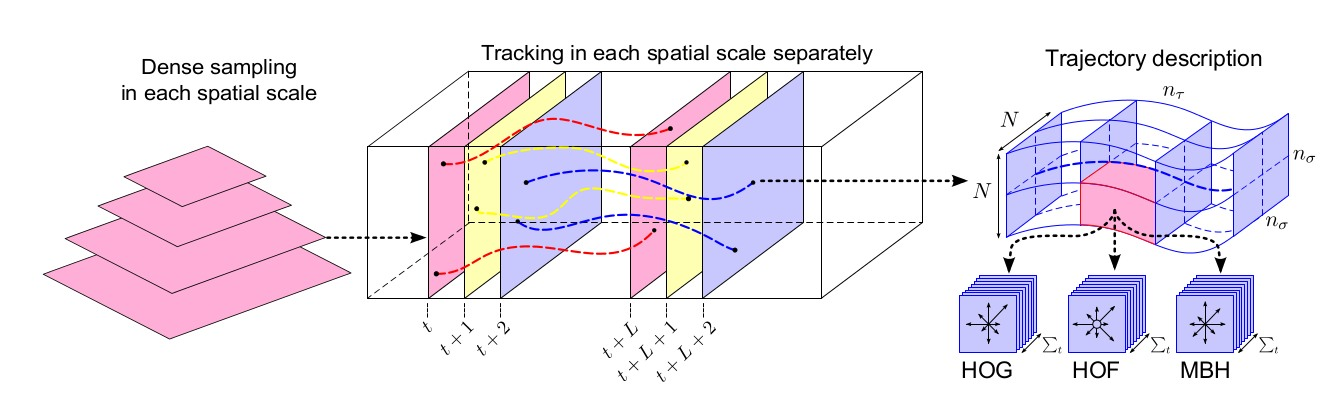
\includegraphics[scale=0.35]{{Images/chap3Dense1}.jpg}}
  \caption{Απεικόνιση της μεθόδου των Πυκνών Τροχιών. $\textbf{Αριστερά}$: Τα σημεία παρακολούθησης δειγματοληπτούνται πυκνά για πολλαπλές χωρικές κλίμακες. $\textbf{Κέντρο}$: Η παρακολούθηση γίνεται στην αντίστοιχη χωρική κλίμακα και για $L$ frames. $\textbf{Δεξιά}$: Οι περιγραφητές τροχιάς βασίζονται στο σχήμα της, που αντιπροσωπεύεται από σχετικές συντεταγμένες σημείων, αλλά και σε πληροφορίες κίνησης και εμφάνισης σε γειτονιές $N \times N$ pixels κατά μήκος της τροχιάς. Προκειμένου να ενσωματωθεί δομική πληροφορία, η κάθε γειτονιά χωρίζεται επιπλέον σε ένα χωρο-χρονικό πλέγμα διαστάσεων $n_{\sigma} \times n_{\sigma} \times n_{\tau}$. Εικόνα από το \cite{wang_2011}.}
  \label{fig:chap3Dense1}
\end{figure}

\par Ξεκινάμε από την πυκνή δειγματοληψία, η οποία εφαρμόζεται σε $8$ κλίμακες ταυτόχρονα και σε ένα τετράγωνο χωρικό πλαίσιο $W \times W$ (δηλαδή με βήμα $W$ σε αμφότερες τις χωρικές διαστάσεις). Πειράματα στο \cite{wang_2011} δείχνουν ότι τιμή $W=5$ είναι επαρκής για την πυκνή δειγματοληψία και ότι περαιτέρω μείωση του $W$ δε συνεισφέρει σημαντικά στην απόδοση του αλγορίθμου παρά επιβαρύνει υπολογιστικά. Σε κάθε πλέγμα απορρίπτουμε τα σημεία που ανήκουν σε ομοιογενείς περιοχές της εικόνας, καθώς είναι αδύνατο να τα παρακολουθήσουμε με χρήση οπτικής ροής. Για το σκοπό αυτό, χρησιμοποιούμε το κριτήριο των Shi-Tomasi \cite{shi_1994}, το οποίο βασίζεται στον ανιχνευτή γωνιών Harris \cite{harris_1988} προκειμένου να εξάγει έναν πίνακα αυτοσυσχέτισης $M(x,y)$, ο οποίος αποτελεί ένα μέτρο της μεταβολής της εικόνας σε κάθε pixel ως προς τις δύο κατευθύνσεις. Αν τώρα $\lambda _1$ και $\lambda _2$ οι ιδιοτιμές του πίνακα αυτού, το κριτήριο γωνιότητας των Shi-Tomasi ελέγχει αν η μικρότερη των δύο ιδιοτιμών αυτών είναι μεγαλύτερη από ένα κατώφλι, το οποίο συχνά επιλέγεται ίσο με $$threshold=0.001\max_{x,y}{(min(\lambda _1,\lambda _2))}$$ Τα σημεία τα οποία δεν ικανοποιούν το κριτήριο Shi-Tomasi απορρίπτονται από την διαδικασία παρακολούθησης.

\par Συνεχίζουμε με την παρακολούθηση των σημείων ενδιαφέροντος. Βασικό συστατικό στην εξίσωση \eqref{eq:pointDense} είναι το πεδίο οπτικής ροής. Η οπτική ροή εκφράζει την σχετική κίνηση κάμερας και σκηνής σε ένα βίντεο. Διαισθητικά εκφράζει τη στιγμιαία ταχύτητα των επιφανειών, ενώ ένα πιο μαθηματικό ανάλογο θα μπορούσαν να αποτελούν τα διανύσματα κατευθυντήριων παραγώγων, κάθετων στις επιφάνειες κίνησης. Η χρήση της οπτικής ροής εδώ έχει σημαντικά πλεονεκτήματα: Αφενός, η μέθοδος παρακολούθησης γίνεται αρκετά πιο εύρωστη από μεθόδους παρεμβολής και αφετέρου, διευκολύνεται ο πυκνός υπολογισμός, αφού μόλις υπολογιστεί η πυκνή οπτική ροή, κάθε σημείο μπορεί να παρακολουθείται χωρίς επιπλέον υπολογιστικό κόστος. Για τον υπολογισμό της οπτικής ροής υπάρχουν αρκετοί αλγόριθμοι \cite{lucas_1981}, αλλά επιλέγεται ο αλγόριθμος του Farneback ως μια συμβιβαστική λύση στο δίλημμα ταχύτητας-ακρίβειας. Συνοπτικά, ο αλγόριθμος αυτός στηρίζεται στην υπόθεση αναπαράστασης της φωτεινότητας εντός πίξελ με ένα πολυωνυμικό ανάπτυγμα του οποίου οι όροι υπολογίζονται με τη μέθοδο των Ελαχίστων Τετραγώνων. Στη συνέχεια, εφαρμόζεται ένας επαναληπτικός αλγόριθμος ο οποίος ελαχιστοποιεί μια συνάρτηση κόστους. To υπολογιστικό πλεονέκτημα αυτού του αλγορίθμου είναι η γρήγορη σύγκλιση και η αποδοτική υλοποίηση, οπότε αρκούν λίγες επαναλήψεις και η οπτική ροή υπολογίζεται ανά δύο frames. Ωστόσο, δεν αξιοποιείται βαθύτερη χωροχρονική πληροφορία κι έτσι θυσιάζεται μικρό μέρος της ακρίβειας.

\par Έχοντας παρακολουθήσει τα σημεία ενδιαφέροντος, τα συνενώνουμε, σχηματίζοντας μια τροχιά. Πειράματα \cite{wang_2011} για το μήκος της τροχιάς δείχνουν καλύτερη λειτουργία για τιμή $15$ με $20$ frames, καθώς μεγαλύτερο μήκος συνεπάγεται μεγαλύτερη πιθανότητα απόκλισης. Το επόμενο βήμα είναι η εξαγωγή των χαρακτηριστικών. Τοπικοί περιγραφητές υπολογίζονται σε έναν τρισδιάστατο χωροχρονικό όγκο γύρω από τα σημεία της τροχιάς, μεγέθους $N \times N$ pixels και $L$ frames, ο οποίος δειγματοληπτείται σε ένα χωροχρονικό πλέγμα $n_{\sigma} \times n_{\sigma} \times n_{\tau}$ προκειμένου να ενσωματώσει δομική πληροφορία στην αναπαράσταση με χαρακτηριστικά. Καλή επιλογή για την τιμή αυτών των παραμέτρων είναι $N=32$, $n_{\sigma}=2$, $n_{\tau}=3$, όπως προκύπτει πειραματικά \cite{wang_2011}. Οι περιγραφητές που υπολογίζονται είναι οι HOF \cite{laptev_2008}, HOG \cite{dalal_2005}, MBH \cite{dalal_2006} και ένας Περιγραφητής Τροχιάς. Ο HΟG περιγράφει το σχήμα και την εμφάνιση γύρω από κάθε τροχιά, ενώ οι HΟF και MBH κωδικοποιούν την κίνηση, με τον τελευταίο μάλιστα να αντισταθμίζει εν μέρει και την κίνηση της κάμερας. Ο Περιγραφητής Τροχιάς κωδικοποιεί απλώς το σχήμα της τροχιάς. Γίνεται επομένως φανερή η συμπληρωματικότητα των περιγραφητών, οι οποίοι κωδικοποιούν διαφορετικά κανάλια πληροφορίας που χαρακτηρίζουν μια δράση. Θα δούμε πώς εκμεταλλευόμαστε το φαινόμενο αυτό στο στάδιο του ταξινομητή, όπου και θα συνδυάσουμε τα διαφορετικά κανάλια. Προς το παρόν, θα αναλύσουμε διεξοδικότερα τη φύση των χαρακτηριστικών που εξάγονται για κάθε τροχιά.


%%%%%%%%%%%%%%%%%%%%%%% Features
\subsection{Είδη Περιγραφητών}

%%%%%%%%%%%% Trajectory Descriptor
\subsubsection{Ο Περιγραφητής Τροχιάς}
Ο περιγραφητής τροχιάς ορίσθηκε στην αυθεντική εργασία των Πυκνών Τροχιών \cite{wang_2011}. Έστω μια τροχιά μήκους $L$ που εκκινεί από το frame $t$. Είναι φανερό ότι μπορούμε να περιγράψουμε το σχήμα της με την ακολουθία των διανυσμάτων μετατόπισης $\Delta P_t=P_{t+1}-P_t$, η οποία θα έχει τη μορφή:

\begin{equation}\label{eq:trajDense}
    S=(\Delta P_{t+1}, \dots ,\Delta P_{t+L-1})
\end{equation}

Ορίζουμε ως περιγραφητή τροχιάς το διάνυσμα που προκύπτει από την κανονικοποίηση της παραπάνω ακολουθίας με το άθροισμα των μέτρων των διανυσμάτων μετατόπισης: 

\begin{equation}\label{eq:trajDescriptor}
    S'=\frac{(\Delta P_{t+1}, \dots ,\Delta P_{t+L-1})}{\sum_{j=t}^{t+L-1} \| \Delta P_j \|}
\end{equation}

Η χρήση του περιγραφητή τροχιάς είναι σημαντική καθώς μοντελοποιεί το σχήμα, το οποίο κωδικοποιεί χαρακτηριστικά της κίνησης. Μάλιστα, στην ίδια εργασία διαπιστώνεται πειραματικά ότι η χρήση μεταβλητού $L$, παρότι σαν ιδέα μπορεί να εκφράσει δράσεις με διαφορετικές ταχύτητες, πρακτικά δε βελτιώνει τα αποτελέσματα, οπότε προτιμάται το σταθερό μήκος τροχιάς.

%%%%%%%%%%%% HOG
\subsubsection{Ιστογράμματα Κατευθυνόμενων Παραγώγων}
Τα Ιστογράμματα Κατευθυνόμενων Παραγώγων (Histograms of Oriented Gradients, εν συντομία HOG) εισήχθησαν στο \cite{dalal_2005} χρησιμοποιούμενα για την αναπαράσταση αντικειμένων στο πρόβλημα της αναγνώρισης αντικειμένων. Η δύναμη του περιγραφητή HOG έγκειται στην αμεταβλητότητά του σε φωτομετρικές και γεωμετρικές μεταβολές, χάρη στην τοπικότητα του υπολογισμού του και των κανονικοποιήσεων που υφίσταται. Η βασική ιδέα είναι η δυνατότητα ικανοποιητικής αναπαράστασης του σχήματος και της εμφάνισης των αντικειμένων σε μια μικρή περιοχή της εικόνας από την κατανομή των τοπικών κλίσεων, δηλαδή των κατευθύνσεων των ακμών στην περιοχή αυτή. Ο υπολογισμός του HOG σε μια γειτονιά περιλαμβάνει τον υπολογισμό τοπικών διακριτών παραγώγων και την κατασκευή των ιστογραμμάτων τους. Περιγράφουμε τη διαδικασία υπολογισμού για εικόνες, ωστόσο είναι φανερό ότι η μέθοδος γενικεύεται σε βίντεο, αν τα θεωρήσουμε ως ένα χωροχρονικό όγκο και μελετήσουμε γειτονιές τριων διαστάσεων.

\begin{figure}
  \centering
  \noindent\makebox[\textwidth]{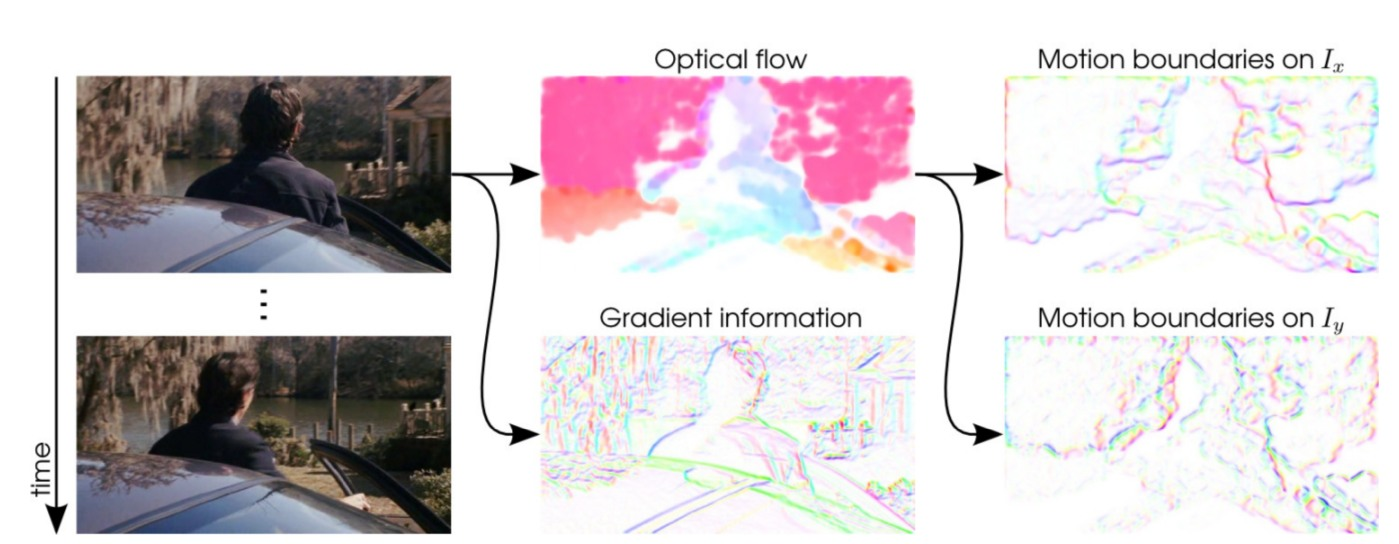
\includegraphics[scale=0.35]{{Images/chap3Features}.jpg}}
  \caption{Απεικόνιση της πληροφορίας που περιέχεται στους περιγραφητές HOG, HOF και MBH. Για κάθε εικόνα, τα διανύσματα κλίσης/οπτικής ροής διακρίνονται με χρώμα (hue) και τα αντίστοιχα μέτρα τους με τη χρωματική συνιστώσα κορεσμού (saturation). Τα όρια κίνησης υπολογίζονται ως παράγωγοι των συνιστωσών $x$ και $y$ της οπτικής ροής ξεχωριστά. Σε σύγκριση με την οπτική ροή, τα όρια κίνησης συμπιέζουν το μεγαλύτερο μέρος της κίνησης του υποβάθρου λόγω κινήσεων της κάμερας και τονίζουν την κίνηση προσκηνίου. Σε αντίθεση με την πληροφορία που λαμβάνεται από τις παραγώγους, τα όρια κίνησης σβήνουν περισσότερη πληροφορία υφής από στατικά παρασκήνια. Εικόνα από το \cite{wang_2011}.}
  \label{fig:chap3Features}
\end{figure}

\par Το πρώτο βήμα της μεθόδου είναι η εφαρμογή του εκθετικού κανόνα (γάμμα διόρθωση) για κωδικοποίηση της φωτεινότητας. Ακολουθεί ο υπολογισμός των παραγώγων της εικόνας με συνέλιξη της εικόνας με τους τελεστές $[-1, 0, 1]$ και $[-1, 0, 1]^T$, μια εύρωστη παραλλαγή της μεθόδου πεπερασμένων διαφορών. Η εικόνα χωρίζεται σε κελιά διάστασης $8 \times 8$ pixels συνήθως και υπολογίζεται το ιστόγραμμα των διευθύνσεων της κλίσης, σταθμισμένο με το αντίστοιχο μέτρο της κλίσης, για τα pixel εντός κάθε κελιού. Κάθε θέση του ιστογράμματος αντιστοιχεί σε μια στάθμη κβάντισης των διευθύνσεων κλίσεων κι έτσι σε ένα μικρό εύρος διευθύνσεων, ανάλογα με το πλήθος των στάθμεων. Τα κελιά ομαδοποιούνται σε μπλοκ (συνήθως $2 \times 2$ κελιών) και τα ιστογράμματα των επιμέρους κελιών συνενώνονται και κανονικοποιούνται σε έναν ενιαίο περιγραφητή. Η συνένωση γίνεται για τη μετρίαση ή μεταφορά της τοπικής σημαντικότητας των pixels σε επίπεδο κελιού στη συνολική σημαντικότητα σε επίπεδο μπλοκ εικόνας, ενώ η κανονικοποίηση γίνεται ώστε να αντισταθμιστούν αλλαγές στη φωτεινότητα και την αντίθεση της εικόνας. Τελικά μια εικόνα περιγράφεται από τη συνένωση των περιγραφητών των μπλοκ που την αποτελούν. Αντίστοιχα σε ένα βίντεο, τα κελιά και τα μπλοκ εκτείνονται σε τρεις διαστάσεις και η λογική είναι παρόμοια.

%%%%%%%%%%%% HOF
\subsubsection{Ιστογράμματα Οπτικής Ροής}
Τα ιστογράμματα οπτικής ροής (Histograms of Optical Flow, εν συντομία HΟF) εισήχθησαν στο \cite{laptev_2008} ως χαρακτηριστικά χρήσιμα στην αναγνώριση δράσεων. Ο περιγραφητής HΟF μοντελοποιεί την κίνηση σε ένα μικρό χωροχρονικό όγκο βίντεο με φιλοσοφία παρόμοια με του  HΟG και χρησιμοποιείται ευρέως σε προβλήματα ανάλυσης και κωδικοποίησης της κίνησης σε βίντεο. Ωστόσο, η διακριτική του ικανότητα εξαρτάται άμεσα από την ακρίβεια της οπτικής ροής. Στην περίπτωση των Πυκνών Τροχιών, ο υπολογισμός των περιγραφητών συνδυάζεται κομψά με τον υπολογισμό της καθαυτής τροχιάς: η οπτική ροή έχει ήδη υπολογιστεί, οπότε ο ίδιος υπολογισμός χρησιμοποιείται στην εξαγωγή των HOF χαρακτηριστικών.
\par Από άποψη υλοποίησης, η πορεία μοιάζει αρκετά με αυτή για τον υπολογισμό του HOG. Συγκεκριμένα, υπολογίζεται αρχικά η οπτική ροή ως προς τους δύο άξονες και κατόπιν το μέτρο και η διεύθυνσή της. Η διεύθυνση κβαντίζεται σε στάθμες με την τελευταία από αυτές να προορίζεται για τα pixels εκείνα στα οποία η οπτική ροή είναι κατά μέτρο μικρότερη από κάποιο κατώφλι. Ακολουθεί, σε πλήρη αντιστοιχία με τον περιγραφητή HOG, η υποδιαίρεση της περιοχής ενδιαφέροντος σε κελιά, για κάθε ένα από τα οποία κατασκευάζεται το ιστόγραμμα των διευθύνσεων της οπτικής ροής. Τα επιμέρους ιστογράμματα ενώνονται και κανονικοποιούνται σχηματίζοντας το τελικό διάνυσμα που περιγράφει την κίνηση εντός του αρχικού όγκου. Προφανώς εδώ γίνεται αντιληπτό το γεγονός ότι ο HOF είναι εγγενώς τρισδιάστατος περιγραφητής, αφού κατασκευάζεται με μεγέθη που αφορούν βίντεο (οπτική ροή).

%%%%%%%%%%%% MBH
\subsubsection{Ιστογράμματα Ορίων Κίνησης}
Τα ιστογράμματα ορίων κίνησης (Motion Boundary Histograms, εν συντομία MBH), εισήχθησαν στο \cite{dalal_2006} με βλέψεις αντιστάθμισης της επίπτωσης της κίνησης της κάμερας στη διακριτική ικανότητα άλλων περιγραφητών που χρησιμοποιούνται για την περιγραφή της κίνησης, όπως ο μεταγενέστερος HOF, οι οποίοι κωδικοποιούν την κίνηση του παρασκηνίου εισάγοντας σημαντικό θόρυβο στην αποτύπωση της πραγματικής κίνησης ενδιαφέροντος. Η ιδέα του MBH είναι η περιγραφή της κίνησης μέσω της παραγώγου της οπτικής ροής προκειμένου να αντισταθμιστεί η κίνηση της κάμερας, εκμεταλλευόμενος την ομοιομορφία της κίνησης λόγω των μεταθέσεων κάμερας έναντι στην τυχαιότητα και τις απότομες μεταβολές που εισάγει μια κίνηση προσκηνίου.

\par Ο υπολογισμός του MBH ξεκινά και πάλι από τον υπολογισμό της οπτικής ροής, που πάλι είναι ήδη υπολογισμένη στην περίπτωση της μεθόδου Πυκνών Τροχιών. Το πεδίο οπτικής ροής χωρίζεται σε οριζόντιο και κατακόρυφο μέρος και υπολογίζεται η παράγωγος για καθένα από αυτά. Η συνέχεια είναι παρόμοια με τη διαδικασία υπολογισμού των HΟG και HOF: η κλίση κβαντίζεται σε στάθμες και εντός ενός κελιού κατασκευάζεται το ιστόγραμμα των κλίσεων σταθμισμένων με το μέτρο τους. Οι δύο περιγραφητές που προκύπτουν (MBHx και ΜΒΗy) κανονικοποιούνται ξεχωριστά και συχνά χρησιμοποιούνται ξεχωριστά, αλλά και σε ενοποιημένη μορφή. Ο MBH είναι αρκετά εύρωστος στην κίνηση της κάμερας, αφού όταν η κίνηση είναι ομαλή, η οπτική ροή περιέχει μια σταθερή συνιστώσα, η οποία αφαιρείται κατά τον υπολογισμό της παραγώγου. Έτσι, κωδικοποιούνται μόνο οι μεταβολές στο πεδίο της οπτικής ροής.


%%%%%%%%%%%%%%%%%%%%%%%%%% Feature Encoding
\subsection{Κωδικοποίηση Χαρακτηριστικών}
Η χρήση των σημείων ενδιαφέροντος εισάγει μια ιδιαιτερότητα στην αναπαράσταση των εικόνων-βίντεο με χαρακτηριστικά: κάθε εικόνα έχει διαφορετικό πλήθος σημείων ενδιαφέροντος κι έτσι διαφορετικό μήκος διανύσματος αναπαράστασης. Τα πράγματα γίνονται ακόμα χειρότερα όταν εισάγονται πολλαπλοί ταξινομητές, καθώς αφενός το μήκος των διανυσμάτων αναπαράστασης ενδέχεται να αλλάζει ακόμα και για την ίδια εικόνα λόγω της κατασκευής του κάθε περιγραφητή, αφετέρου οι τιμές των χαρακτηριστικών περιέχουν τελείως διαφορετική και ανεξάρτητη πληροφορία μεταξύ τους, οπότε η ενιαία αναπαράσταση και σύγκριση δεν έχει κάποια ερμηνεία. Έτσι, παρόλο που η συμπληρωματική φύση των περιγραφητών ωφελεί τα χαρακτηριστικά και αυξάνει τη διαχωρισιμότητα των κλάσεων, απαιτείται κωδικοποίηση για την αποτελεσματική τους χρήση. Μια επιτυχής λύση στο πρόβλημα αυτό είναι η κωδικοποίηση με τη μέθοδο του «σάκου λέξεων» (bag-of-words). Η ιδέα είναι εμπνευσμένη από την κατηγοριοποίηση κειμένου, ενός χώρου όπου το πρόβλημα είχε εμφανιστεί εγγενώς στο παρελθόν. Εκεί το πρόβλημα είναι η μοντελοποίηση προτάσεων διαφορετικού μήκους με έναν ενιαίο τρόπο. Τελικά, αντί να αναπαριστούμε τις προτάσεις με τις λέξεις τους, τις αναπαριστούμε με την κατανομή των λέξεων και μάλιστα κατασκευάζουμε ένα λεξικό μέ τις λέξεις των προτάσεων του συνόλου εκπαίδευσης και μετράμε την εμφάνιση ή μη αυτών των λέξεων σε κάθε νέα πρόταση. Φυσικά υπάρχουν και πιο σύνθετες αναπαραστάσεις \cite{jones_1972}, αλλά αυτή που περιγράφηκε είναι η πιο σχετική με τη λύση στα προβλήματα Όρασης Υπολογιστών. Θα δούμε τώρα πώς, συσχετίζοντας τα προβλήματα αναπαράστασης γλωσσικών προτάσεων και βίντεο, μπορούμε να εξάγουμε ανάλογη λύση.

\begin{figure}
  \centering
  \noindent\makebox[\textwidth]{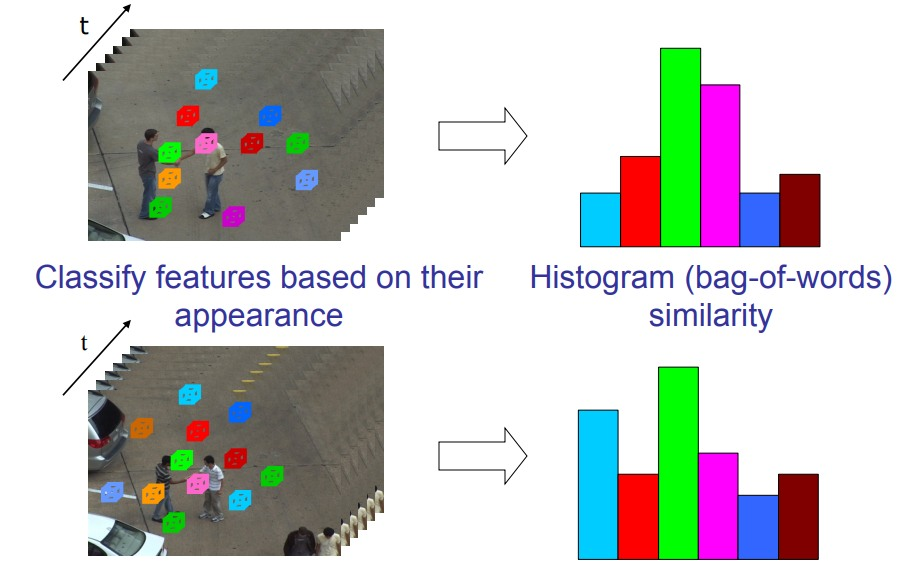
\includegraphics[scale=0.3]{{Images/chap3BOW}.jpg}}
  \caption{Απεικόνιση της μεθόδου του Σάκου Οπτικών Λέξεων (Bag of Visual Words, εν συντομία BoW). Οι διαφορετικοί τύποι χαρακτηριστικών εξάγονται σε σημεία ενδιαφέροντος στο βίντεο. Στη συνέχεια κωδικοποιούνται για να σχηματίσουν ένα λεξιλόγιο, τον Σάκο Λέξεων. Ένα βίντεο τώρα αναπαρίσταται σαν μια πρόταση από οπτικές λέξεις και ταξινομείται σύμφωνα με το ιστόγραμμα των λέξεων αυτών. Μια απλή περίπτωση είναι η ταξινόμηση απευθείας σύμφωνα με τα ιστογράμματα αυτά. Στην πορεία αυτής της εργασίας θα δούμε αρκετά πιο σύνθετες μεθόδους. Εικόνα από το \cite{cvpr_2011}.}
  \label{fig:chap3BOW}
\end{figure}

\par Μπορούμε να σκεφτούμε μια εικόνα ή ένα βίντεο σαν μια οπτική πρόταση, σε αναλογία με την γλωσσική πρόταση. Η αναλογία αυτή διατηρεί την ποικιλομορφία και το μεταβλητό μέγεθος, ωστόσο υπάρχει ένα λεπτό σημείο που πρέπει να διευκρινιστεί για να είναι η αναλογία έγκυρη: το σύνολο των λέξεων που σχηματίζουν κάθε πρόταση. Από τη μία μεριά το σύνολο των γλωσσικών λέξεων είναι αριθμήσιμο (μπορούμε να σκεφτούμε ότι κάθε λέξη είναι μια μετάθεση ενός συνδυασμού των γραμμάτων του αλφαβήτου), ενώ, από την άλλη, δεν έχουμε ορίσει σύνολο οπτικών λέξεων. Η ιδέα να ορίσουμε ως λέξη ένα ιστόγραμμα χαρακτηριστικών απορρίπτεται καθώς οι τιμές των οπτικών χαρακτηριστικών απεικονίζονται σε έναν συνεχή χώρο, την στιγμή που ζητάμε ένα αριθμήσιμο σύνολο. Το πρώτο βήμα επομένως, είναι η κβάντιση του συνόλου οπτικών χαρακτηριστικών για τη δημιουργία ενός οπτικού λεξικού. Συνήθως αυτή η διαδικασία εφαρμόζεται χωριστά σε κάθε περιγραφητή, αφού, όπως εξηγήσαμε, η σύγκριση τιμών διαφορετικών περιγραφητών δεν έχει καμία φυσική έννοια.

\par Το οπτικό λεξικό για κάθε περιγραφητή θα προκύψει από έναν αλγόριθμο ομαδοποίησης. Η μέθοδος των Πυκνών Τροχιών, όπως προτάθηκε στην αυθεντική της μορφή, υπολογίζει λεξικά μεγέθους $4000$ λέξεων για κάθε περιγραφητή που χρησιμοποιεί, τρέχοντας τον αλγόριθμο k-μέσων (k-means) \cite{steinhaus_1956}. Ο k-means είναι ίσως ο δημοφιλέστερος αλγόριθμος διανυσματικής κβάντισης και χρησιμοποιείται για να διαιρέσει τον αρχικό χώρο X των χαρακτηριστικών σε $k$ περιοχές, κάθε μια από τις οποίες αντιπροσωπεύεται από ένα διάνυσμα $d_i\in D = d_1, \dots , d_k$, όπου $D$ τα κεντροειδή του k-means, δηλαδή το οπτικό λεξικό. Για τον υπολογισμό των κέντρων $D$, ο k-means εκκινεί από αρχικοποιημένες τιμές $k$ κέντρων $m_1^{(1)}, \dots\, m_k^{(1)}$ και επαναλαμβάνει τα εξής δύο βήματα:

\begin{equation}\label{eq:kmeansAssign}
    \text{Assignment Step: } \text{ } S_i^{(t)}=\{ x_p: \| x_p-m_i^{(t)}\| \leq \| x_p-m_j^{(t)}\|  \forall j, \text{ } 1 \leq j \leq k \}
\end{equation}

και

\begin{equation}\label{eq:kmeansUpdate}
    \text{Update Step: } \text{   } m_i^{(t+1)}=\frac{1}{| S_i^{(t)} |} \sum_{x_j \in S_i^{(t)}} x_j
\end{equation}

Οι επαναλήψεις σταματούν όταν δεν υπάρχει άλλη ανανέωση. Με άλλα λόγια, λύνεται ένα πρόβλημα ομαδοποίησης όπου κάθε διάνυσμα αντιστοιχίζεται στην κλάση του κοντινότερού του μέσου. Η προσθήκη ενός νέου διανύσματος σε μια κλάση επηρεάζει το μέσο διάνυσμα της κλάσης αυτής (και της κλάσης από την οποία αφαιρείται), οπότε επανεκτιμουμε την ανάθεση των υπολοίπων διανυσμάτων σε αυτή τη νέα κλάση. Αναφέρεται βέβαια ότι ο αλγόριθμος δεν εγγυάται βέλτιστη διαμέριση του χώρου.

\par Έχοντας κατασκευάσει το οπτικό λεξικό, πρέπει να κωδικοποιήσουμε τα οπτικά χαρακτηριστικά ώστε να τα μετατρέψουμε σε οπτικές λέξεις. Η διαδικασία εδώ είναι απλή: κάθε χαρακτηριστικό αντιστοιχίζεται στην λέξη που αντιστοιχεί στο κοντινότερο (υπό κάποια μετρική απόστασης, στη μέθοδο Πυκνών Τροχιών χρησιμοποιείται η Ευκλείδεια απόσταση) κεντροειδές του οπτικού λεξικού. Έτσι το πρόβλημα διακριτότητας των λέξεων έχει λυθεί. Όπως στην περίπτωση των γλωσσικών προτάσεων, έτσι και μια οπτική πρόταση αντιπροσωπεύεται από την κατανομή (εμφάνιση ή μη και συχνότητα) των λέξεων που την αποτελούν, πάνω στο, κατασκευασμένο κατά τη διάρκεια εκπαίδευσης, οπτικό λεξικό, δηλαδή λαμβάνουμε το ιστόγραμμα των λέξεων της πρότασης. Στην περίπτωση των βίντεο, αυτή η αναπαράσταση συμβαίνει σε κάθε frame και για την αναπαράσταση όλου του τμήματος βίντεο λαμβάνουμε το αθροιστικό ιστόγραμμα πάνω στα επιμέρους frames που το αποτελούν. Ωστόσο αυτή η επιλογή παρουσιάζει δύο ακόμα προκλήσεις. Αρχικά, μια πρόταση έχει μεταβλητό μέγεθος. Επομένως τα ιστογράμματα θα εμφανίζουν μεγάλες διακυμάνσεις στις τιμές τους ακόμα και στην αναπαράσταση της ίδιας δράσης. Μας ενδιαφέρει η κατανομή κι όχι το μήκος της πρότασης, οπότε λαμβάνουμε τα κανονικοποιημένα ιστογράμματα οπτικών λέξεων. Τώρα η αναπαράσταση είναι ενιαία και ανεξάρτητη του μήκους βίντεο ή γλωσσικής πρότασης. Η δεύτερη πρόκληση αφορά την απαλοιφή της χωροχρονικής συσχέτισης μεταξύ των λέξεων. Πράγματι, τόσο στην περίπτωση των γλωσσικών όσο και των οπτικών προτάσεων, η εξαγωγή του ιστογράμματος βασίζεται στην εμφάνιση και μόνο μιας λέξης κι όχι τη χωρική της σχέση με τις υπόλοιπες λέξεις. Παρότι υπάρχουν μέθοδοι που μπορούν να αποδώσουν κάποια χωρική σχέση (όπως τα n-grams στην περίπτωση των γλωσσικών προτάσεων), η απόδοση των μεθόδων BoW είναι υψηλή, οπότε συνεχίζουν να χρησιμοποιούνται.


%%%%%%%%%%%%%%%%%%%%%%%%%%%%% Pose Features
\subsection{Επιπλέον Χαρακτηριστικά: Τα Χαρακτηριστικά Πόζας}
Στο \cite{rohrbach_2012} εισάγεται μια επέκταση της μεθόδου Πυκνών Τροχιών, η οποία λαμβάνει υπόψιν της περισσότερα χαρακτηριστικά. Οι συγγραφείς χρησιμοποιούν επιπλέον χαρακτηριστικά της στάσης του άνω τμήματος του σώματος. Το κίνητρο πίσω από αυτό το εγχείρημα είναι η αίσθηση ότι οι λεπτομερείς δραστηριότητες αφορούν κυρίως τα χέρια και τις κινήσεις των άνω μερών του σώματος. Σε πρώτη φάση εξάγεται η στάση του σώματος και υπολογίζονται οι τροχιές στάσης στα βίντεο. Γύρω από τις τροχιές εξάγονται χαρακτηριστικά πόζας τα οποία κωδικοποιούνται και μπορούν να αναπαραστήσουν τη δράση. Περιγράφουμε τώρα αναλυτικότερα τα επιμέρους βήματα του αλγορίθμου.

\begin{figure}
  \centering
  \noindent\makebox[\textwidth]{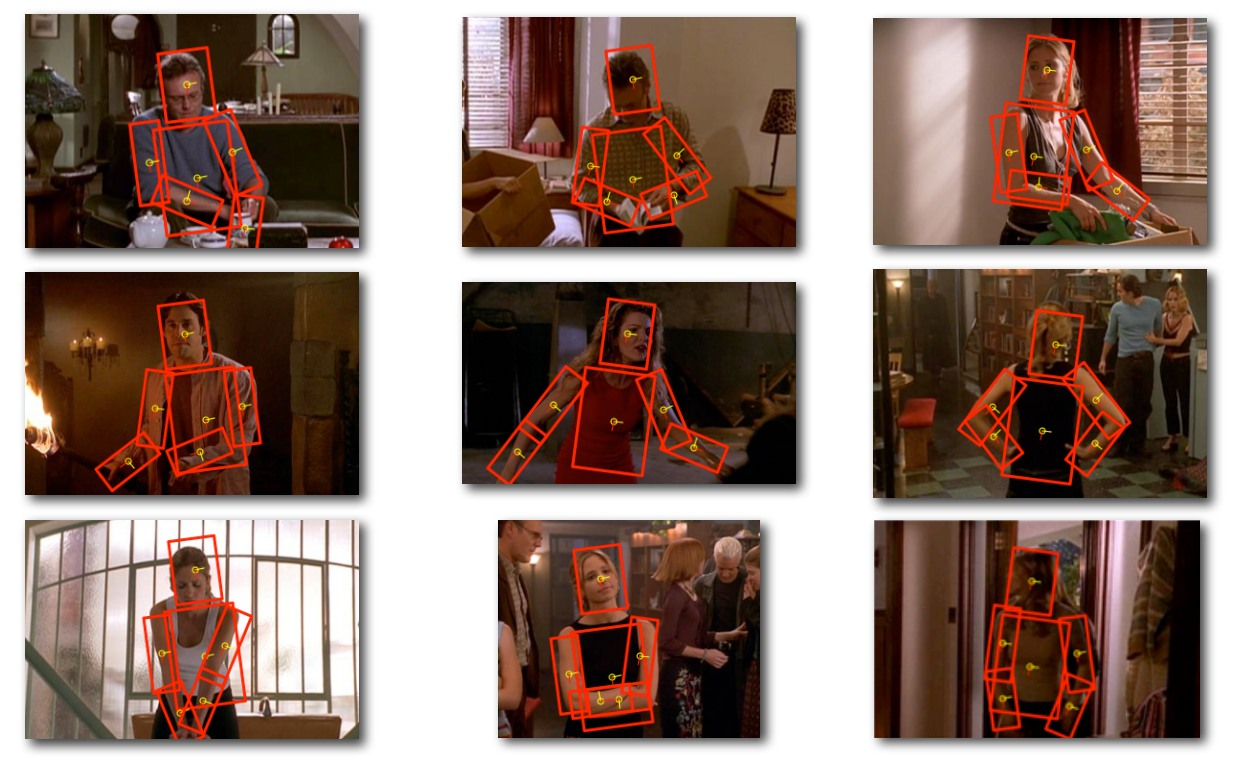
\includegraphics[scale=0.3]{{Images/chap3Poses}.jpg}}
  \caption{Μερικά παραδείγματα επιτυχούς ανίχνευσης στάσης του άνω ήμισυ του σώματος. Η στάση μπορεί να σχετίζεται άμεσα με την δράση. Ιδιαίτερα η θέση και ο σχηματισμός των χεριών αποτελούν σημαντικό διακριτικό στοιχείο των λεπτομερών δράστηριοτήτων. Εικόνα από το \cite{andriluka_2009}.}
  \label{fig:chap3Poses}
\end{figure}

\par Το πρώτο βήμα είναι η εκτίμηση της στάσης του σώματος. Για το σκοπό αυτό, οι συγγραφείς χρησιμοποιούν τον εκτιμητή πόζας του \cite{andriluka_2009}. Η εργασία αυτή βασίζεται στις Εικονικές Δομές (Pictorial Structures, εν συντομία PS) \cite{felzenszwalb_2005} και σε ισχυρούς ανιχνευτές τμημάτων, όπως των \cite{mikolajczyk_2006} και \cite{viola_jones}. Πιο συγκεκριμένα, γίνεται χρήση περιγραφητών σχήματος \cite{mikolajczyk_2005} για την εξαγωγή πυκνών αναπαραστάσεων και εκπαιδεύονται ταξινομητές παραμορφώσιμων τμημάτων με τον αλγόριθμο AdaBoost \cite{freund_1997}. Οι έξοδοι των ταξινομητών αυτών συνδυάζονται με ένα μοντέλο PS, σύμφωνα με τα σκορ του ταξινομητή. Καθώς ο αλγόριθμος είναι γενικός και απευθύνεται σε οποιοδήποτε σύνολο δεδομένων, οι συγγραφείς του \cite{rohrbach_2012} εκπαιδεύουν ένα μοντέλο αποκλειστικά για το δικό τους σύνολο δεδομένων. Ο αλγόριθμος τροποποιείται ελαφρά ώστε να χρησιμοποιεί 10 αντί για 6 τμήματα του σώματος. Τα αποτελέσματα εκτίμησης πόζας βελτιώνονται αισθητά μετά τη νέα εκπαίδευση, καθώς το μοντέλο προσαρμόζεται στο σύνολο δεδομένων.

\par Έχοντας υπολογίσει την πόζα με τον παραπάνω αλγόριθμο, χρειαζόμαστε χρονική πληροφορία, δηλαδή την τροχιά των συνδέσμων του σώματος. Για εξοικονόμηση υπολογισμών, εκμεταλλευόμενοι την πυκνότητα του συνόλου δεδομένων μπορούμε να υπολογίσουμε την στάση του σώματος ανά $10$ frames και να την παρακολουθήσουμε σε ένα χρονικό πλαίσιο $100$ frames με κέντρο το κάθε ένα από τα frames στα οποία έχει γίνει η εκτίμηση. Για την παρακολούθηση (tracking), χρησιμοποιείται ο αλγόριθμος SIFT \cite{lowe_1999}. Η παρακολούθηση γίνεται για κάθε σύνδεσμο ξεχωριστά και τα αποτελέσματα των διαφορετικών κέντρων παρακολούθησης συνεκτιμώνται. Μάλιστα γίνεται επιλογή των χαρακτηριστικών που παρουσιάζουν τη μέγιστη συνεκτική κίνηση για κάθε σύνδεσμο και η θέση ανανεώνεται μόνο σύμφωνα με αυτά τα χαρακτηριστικά για την αποκοπή outliers. Το πλεονέκτημα αυτής της προσέγγισης είναι ο συνδυασμός ενός γενικού μοντέλου εμφάνισης με ένα μοντέλο ειδικής εμφάνισης όπως αυτό που παρακολουθεί ο αλγόριθμος SIFT.

\par Η εξαγωγή των τροχιών στάσης σώματος ανοίγει το δρόμο για τον υπολογισμό των χαρακτηριστικών πόζας. Πρώτα χαρακτηριστικά είναι αυτά του Μοντέλου Σώματος (Body Model, εν συντομία BM). Η διαδικασία υπολογισμού αυτών των χαρακτηριστικών εκκινεί με τον υπολογισμό των ταχυτήτων και των επιταχύνσεων για όλους τους συνδέσμους και την κβάντισή τους σε ιστογράμματα $8$ θέσεων. Ο διαχωρισμός γίνεται με βάση την κατεύθυνση του διανύσματος σταθμισμένη με τον αριθμό των pixels ανά frame. Επιπλέον, υπολογίζονται οι αποστάσεις μεταξύ των αντίστοιχων συνδέσμων (αριστερού-δεξιού) και των διαφόρων κατηγοριών συνδέσμων του άνω μέρους του σώματος μεταξύ τους. Για κάθε μία από τις τροχιές αυτών των αποστάσεων υπολογίζονται στατιστικά (μέση τιμή, διάμεσο, τυπική απόκλιση, μέγιστο και ελάχιστο) και ιστογράμματα παρόμοια με αυτά της ταχύτητας και της επιτάχυνσης. Τέλος, υπολογίζονται οι τροχιές και γωνιών και των γωνιακών ταχυτήτων όλων των εσωτερικών σημείων (καρπών, αγκώνων και ώμων) και γίνεται εξαγωγή στατιστικών για αυτές. Δεύτερα χαρακτηριστικά που εξάγονται γύρω από τις τροχιές πόζας είναι τα χαρακτηριστικά FFT, εμπνευσμένα από την επιτυχία τους στο \cite{zinnen_2009}. Τα χαρακτηριστικά αυτά περιέχουν $4$ εκθετικές ζώνες, $10$ συντελεστές Cepstrum και την φασματική εντροπία και ενέργεια για κάθε συντεταγμένη $x$ και $y$ των τροχιων όλων των συνδέσμων.

\par Παρότι η αυθεντική μέθοδος των Πυκνών Τροχιών απορρίπτει το μεταβλητό μήκος τροχιάς λόγω της χαμηλής του προσφοράς στο τελικό αποτέλεσμα, η ιδέα εφαρμόζεται τελικά στα χαρακτηριστικά πόζας. Συγκεκριμένα, κάθε είδος χαρακτηριστικού (BM, FFT) κωδικοποιείται ξεχωριστά. Για τρία διαφορετικά μήκη τροχιάς (20, 50, 100 frames) με κέντρο το frame όπου έγινε η ανίχνευση εξάγονται το χαρακτηριστικά και συνενώνονται για να αναπαραστήσουν με μεγαλύτερη επιτυχία δράσεις με διαφορετικό μήκος. Η κωδικοποίηση γίνεται με μέγεθος λεξιλογίου διπλάσιο του μήκους κάθε διανύσματος χαρακτηριστικών για κάθε μία από τις δύο κατηγορίες χαρακτηριστικών. Με αυτόν τον τρόπο, έχουμε αναπαραστήσει κάθε δράση και με κίνηση συνδέσμων και στάση σώματος.


%%%%%%%%%%%%%%%%%%%%%%%%%%%%%%%%%%%%%%%%%%%%%% Our Design
\section{Προτεινόμενο Σύστημα}
Συνοψίζοντας όσα παρουσιάσαμε παραπάνω, η προσέγγισή μας συνδυάζει όλη την πορεία από την παρακολούθηση του βίντεο και την εξαγωγή χαρακτηριστικών μέχρι την κωδικοποίησή τους σε ιστογράμματα. Διατηρήσαμε τις ήδη ορισμένες (default) τιμές παραμέτρων όπου χρειάστηκε. Συγκεκριμένα, σε πρώτη φάση εξαγάγαμε τα χαρακτηριστικά HOG, HOF, MBH (σε ενιαία, μετρική μορφή) και Περιγραφητή Τροχιάς, καθώς και τα χαρακτηριστικά πόζας BM και FFT. Στη φάση της κωδικοποίησης, τρέξαμε τον αλγόριθμο k-μέσων για τη δημιουργια λεξιλογίων (codebooks) πλήθους 4000 για τα χαρακτηριστικά των τροχιών (HOG, HOF, ΜΒΗ, Περιγραφητή Τροχιάς), 3336 για τα χαρακτηριστικά ΒΜ και 1536 για τα χαρακτηριστικά 1536 FFT. Αφού λάβαμε τα ιστογράμματα των χαρακτηριστικών ελέγξαμε ποικίλλους τρόπους συνδυασμού πριν την ταξινόηση, ώστε να αποκομίσουμε τα μέγιστα οφέλη από τη συμπληρωματική φύση των χαρακτηριστικών. Αφήνουμε όμως τα πειράματα αυτά για το κεφάλαιο 6, αφού θα έχουμε εξάγει τα ιστογράμματα από τα υπόλοιπα κανάλια πληροφορίας.

\begin{figure}
  \centering
  \noindent\makebox[\textwidth]{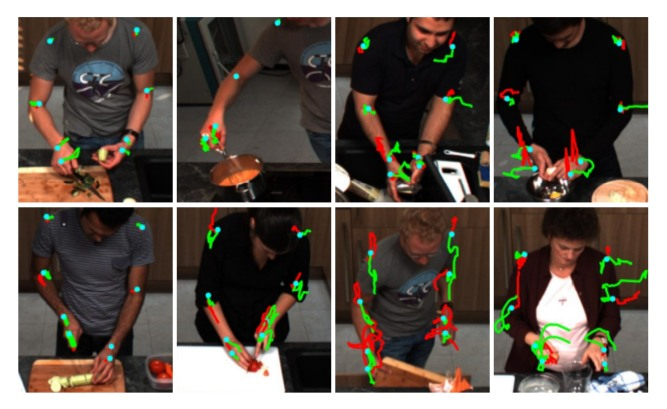
\includegraphics[scale=0.5]{{Images/chap3Tracks}.jpg}}
  \caption{Μερικά παραδείγματα εξαγωγής εμπροσθόδρομων και οπισθόδρομων τροχιών των 10 τμημάτων του άνω μισού μέρους του σώματος κατά την παρακολούθησή τους στην εξαγωγή των χαρακτηριστικών πόζας. Με πράσινο απεικονίζονται οι οπισθόδρομες μετακινήσεις και με κόκκινο οι εμπροσθόδρομες. Με κυανό σημειώνεται η αρχική θέση του κάθε συνδέσμου. Εικόνα από το \cite{rohrbach_2012}.}
  \label{fig:chap3Tracks}
\end{figure}

\end{document}
